\documentclass[a4paper,12pt,titlepage]{article}
%packages
\usepackage[utf8]{inputenc}
\usepackage{geometry}
\usepackage{german}
\usepackage{amssymb}
\usepackage{url}
\usepackage{graphicx}
\usepackage{setspace}
\usepackage{eurosym}
\usepackage{tabularx}
\usepackage{amsmath}

 %settings
\geometry{a4paper,left=30mm,right=25mm, top=20mm, bottom=20mm}
\onehalfspacing
\bibliographystyle{plain}
\author
{
Niklas Gögge\\
Viktoriaschule Aachen\\
Kurs: Mathematik(LK)\\
Fachlehrerin: Frau Kleines\\
Schuljahr 2014/15
}


%document beginns here
\begin{document}
\begin{titlepage}
\begin{center}

\LARGE Asymmetrische Verschlüsselungsverfahren am Beispiel vom Merkle-Hellman-Kryptosystem

\vspace{2cm}
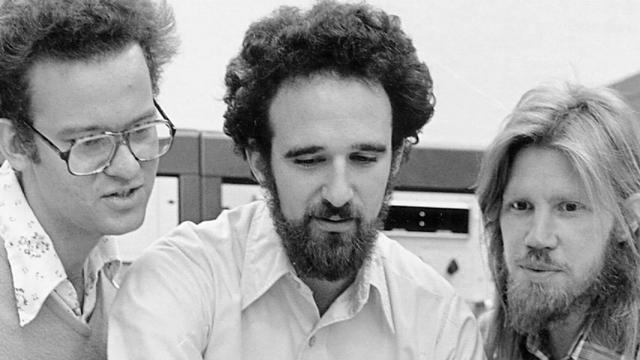
\includegraphics[scale=0.4,natwidth=640,natheight=360]{titlepicture.jpg} \\
\vspace{2cm}

\large
Niklas Gögge\\
Viktoriaschule Aachen\\
Kurs: Mathematik(LK)\\
Fachlehrerin: Frau Kleines\\
Schuljahr 2014/15 \\
\vspace{1cm}
8. März 2015
\end{center}
\end{titlepage}

\newpage

\tableofcontents

\newpage

\section{Einleitung}
Diese Facharbeit entsteht im Rahmen einer Schulaufgabe im Leistungskurs Mathematik und
beschäftigt sich mit asymmetrischen Verschlüsselungsverfahren am Beispiel vom
Merkle-Hellman-Kryptosystem (\cite{merklehellman_neer}). Ich habe dieses Thema
gewählt, da ich sehr mathematisch und informationstechnisch interessiert bin
und mein späteres Studium wahrscheinlich auch in eine dieser Richtungen
verlaufen wird. Des
Weiteren sind Sicherheit und Geheimhaltung im heutigen Medienzeitalter ein sehr
interessantes und vor allem wichtiges Thema, da ein sehr großer Teil der
Kommunikation über Telefone beziehungsweise über das Internet läuft.

Die Ziele dieser Arbeit sind, beim Leser ein grundsätzliches Verständnis über
Verschlüsselung im Allgemeinen zu vermitteln und im Besonderen asymmetrische
Verschlüsselung am Beispiel des Merkle-Hellman-Kryptosystems näher zu
beleuchten.

Für das grundsätzliche Verständnis dienen die Kapitel \ref{math}-\ref{asymm}.
Dabei werden zunächst die mathematischen Grundlagen, die für das Verständnis
der Arbeit gebraucht werden, erläutert. Dazu gehören: Restrechnung, der
euklidische Algorithmus, der erweiterte euklidische Algorithmus,
Einwegfunktionen mit und ohne Falltür sowie stark wachsende Vektoren. Das
darauf folgende Kapitel beschäftigt sich allgemein mit Verschlüsselung, ihre
Ziele, Verschlüsselungsprotokolle und ihre Anwendungsbereiche. Die zwei
folgenden Kapitel informieren über symmetrische und asymmetrische
Verschlüsselung, ihre Prinzipien und deren Sicherheit. Kapitel \ref{mhk}
erläutert, als Beispiel für ein asymmetrisches Verfahren, das
Merkle-Hellman-Kryptosystem. Dazu gehören: eine kurz Biographie der Erfinder,
das Rucksackproblem, das angewandte Verfahren an sich (Schlüsselerzeugung,
Verschlüsselung, Entschlüsselung) und die Sicherheit des Verfahrens. Zum
Schluss habe ich noch ein persönliches Fazit aus meiner Bearbeitung dieser
Arbeit gezogen.

Ergänzend habe ich im Rahmen dieser Arbeit
das Merkle-Hellman-Kryptosystem in der Programmiersprache Java selber
programmiert.

\newpage

\section{Mathematische Grundlagen}\label{math}

Der Kern jedes Verschlüsselungssystems sind mathematische Grundlagen. Für den Umfang dieser Arbeit wird lediglich auf einige eingegangen. Dabei wird die Restrechnung, der euklidische Algorithmus und der erweiterte euklidische Algorithmus, die Einwegfunktionen sowie stark wachsende Vektoren beschrieben, um in den nachfolgenden Kapiteln darauf aufzubauen.

\subsection{Restrechnung}
Die Restrechnung ist den meisten vermutlich noch aus der Grundschule bekannt, denn bevor rationale Zahlen eingeführt wurden, war zum Beispiel: 123 geteilt durch 10 nicht etwa 12.3, sondern das Ergebnis lautete: 12 Rest 3. Allgemein ausgedrückt heißt es, dass bei einer Division zweier Zahlen $a,b$, mit $b \neq 0$, $a,b \in \mathbb{Z}$ ein Rest $r$ entstehen kann. Eine mögliche Schreibweise dafür wäre:
\begin{center}
$r = a \; mod \; b$
\end{center}
Auf das obige Beispiel bezogen würde man also $3 = 123 \; mod \; 10$ schreiben.\footnote{Die Schreibweise für modulo ist $mod$.} \newline Bei Restrechnung geht es auch oft um Restklassen. Eine Restklasse besteht immer aus Zahlen, welche geteilt durch eine Zahl $b$, mit $b \in \mathbb{Z}$, den selben Rest ergeben. So sind zum Beispiel die Zahlen 2; 5; 11; 38; 41; 86; 101 alle ein Teil der Restklasse modulo 3, denn sie alle ergeben bei der Division durch 3 den gleichen Rest. Im Zusammenhang mit Restklassen wird auch oft von Kongruenz geredet. Zwei Zahlen $a, b$ sind kongruent zueinander, wenn sie dividiert durch eine dritte Zahl $c$ den selben Rest $r$ überlassen. Die Schreibweise dafür ist:
 \begin{center}
$a \equiv b \; mod \; c$
 \end{center}
Ausgesprochen heißt das: $a$ ist kongruent $b$ modulo $c$.
Das heißt also, dass alle Zahlen einer Restklasse kongruent zueinander sind.

\subsection{Euklidischer Algorithmus}
Viele asymmetrische Verschlüsselungsverfahren müssen häufig den größten gemeinsamen Teiler oder kurz den ggT\footnote{Der ggT zweier Zahlen ist die größte mögliche Zahl, durch welche beide teilbar sind.} zweier oder mehrerer Zahlen errechnen und der euklidische Algorithmus ist nichts anderes als eine Methode um dies zu tun. Er erhielt seinen Namen von seinem Erfinder Euklid.\newline Um den ggT zweier ganzer Zahlen $a, b$ mit $a > b$ zu bestimmen, wird zuerst $c = a \; mod \; b$ berechnet. Dann wird der Wert von $a$ in den von b geändert und der von $b$ in den von $c$. Danach wird dieser Vorgang mit ''neuem'' $a$ und $b$ wiederholt solange bis $c$ gleich 0 ist. Und dann ist der letzte von $b$ angenommene Wert, der ggT von $a$ und $b$.
Wenn der $ggT(a, b) = 1$, dann sind $a$ und $b$ teilerfremd.

\subsection{Erweiterter Euklidischer Algorithmus}\label{exteuk}
Der erweiterte euklidische Algorithmus bestimmt zusätzlich zum ggT von zwei ganzen Zahlen $a,b$ mit $b \neq 0$ noch zwei weitere ganze Zahlen $s,t$. Die Gleichung, die dabei gelöst wird, ist folgende:
\begin{center}
$ggT(a,b) = s \cdot a + t \cdot b$
\end{center}
Hier wird der Algorithmus an einem Beispiel erklärt:
\begin{quote}
\glqq Der Algorithmus sieht wie folgt aus:  \\
i. $m = a, n = b, s = 1, t = 0, u = 0, v = 1$ \\
ii. Berechne $q$ und $r$ mit $m = q\cdot n + r$ (Division mit Rest) \\
iii. Setze $m = n, n = r, u'=s - q \cdot u, v'= t-q \cdot v$\\
iv. Setze $s=u, t=v,u=u',v=v'$ \\
v. Falls $n>0$ gehe zu Schritt (ii) \\
Nach Beendigung $ggT(a,b) = m = s \cdot a + t \cdot b$. \\[1\baselineskip]

Beispiel\\
Für $a = 37$ und $b = 16$ ergibt sich: \\
$37 = 1 \cdot 37 + 0 \cdot 16$\\
$16 = 0 \cdot 37 + 1 \cdot 16 (q=2)$\\
$5 = 1 \cdot 37 - 2 \cdot 16 (q=3)$\\
$1 = (-3) \cdot 37 + 7 \cdot 16 (q=5)$\\
$0 = 16 \cdot 37 - 37 \cdot 16$.\\
Also ist $ggT(a,b) = 1 = (-3) \cdot 37 + 7 \cdot 16$.\grqq{} (\cite{exteuk} Beschreibung des Algorithmus)
\end{quote}
Die häufigste Anwendung dieses Algorithmus in der Verschlüsselung ist die Bestimmung von multiplikativen Inversen. Zwei ganze Zahlen $a, b$ haben multiplikative Inverse, wenn sie teilerfremd sind.
Das Inverse zu $a$ also $a^{-1}$ ist $s$ und das Inverse zu $b$ also $b^{-1}$ ist $t$. (\cite{exteuk})

\subsection{Einwegfunktionen}
Eine Einwegfunktion ist eine Funktion welche leicht zu berechnen ist. Es ist also $y = f(x)$ schnell zu  berechnen, aber es ist nur sehr schwer bis unmöglich die Funktion umzukehren, also $x = f^{-1}(x)$ ist nicht effizient zu berechnen. Es wird angenommen, dass solche Funktionen existieren und es gibt auch einige Funktionen bei denen man annimmt, dass es sich um Einwegfunktionen handelt, allerdings ist dies nicht bewiesen. Einwegfunktionen werden vor allem in der asymmetrischen Verschlüsselung häufig angewendet, allerdings wird dort eine spezielle Art von Einwegfunktionen verwendet, die so genannten Einwegfunktionen mit Falltür. (\cite{oneway_lukas} 1.2 Einwegfunktionen)

\subsubsection{Einwegfunktionen mit Falltür} \label{oneway_trapdoor}
Einwegfunktionen mit Falltür sind Einwegfunktionen mit einer zusätzlichen Eigenschaft. Sie sind umkehrbar, allerdings nur mit den richtigen Falltür- /Geheiminformationen. (\cite{oneway_lukas} 2.2 Einwegfunktionen mit Falltür)

\subsubsection{Beispiel}
Ein Beispiel für eine Einwegfunktion ist die Multiplikation zweier Primzahlen.
Eine solche Funktion könnte $f(a,b) = a \cdot b$ lauten. \newline Wählt man jetzt zum Beispiel $a = 37967$ und $b = 41389$, so ist das Ergebnis von $f(37967, 41389)$ die Zahl 1571416163. Das Multiplizieren von $a$ und $b$ geht schnell, also ist die erste Bedingung einer Einwegfunktion erfüllt und ohne weiteres ist es auch nicht leicht aus dem Ergebnis die beiden Primzahlen $a,b$ herauszuziehen, außer eine der beiden ist bekannt und somit ist die zweite Bedingung der Definition auch erfüllt. Allerdings kann ein Computer in diesem Fall $a,b$ trotzdem schnell errechnen, da $a,b$ sehr klein sind. Wählt man $a,b$ sehr groß, so ist es praktisch unmöglich aus dem Ergebnis die beiden Primzahlen zu zerlegen. Diese Einwegfunktion wird vom RSA-Kryptosystem verwendet, welches in dieser Arbeit allerdings nicht erläutert wird.

\subsection{Stark wachsende Vektoren}
Ein stark wachsender Vektor $V$ ist eine Abfolge von Zahlen, in der jede nächste Zahl $V[k]$ größer ist als die Summe aller Zahlen zuvor. Für $k > 0$ heißt das mathematisch ausgedrückt:
\begin{equation*}
V[k] > \sum_{i = 0}^{k - 1}V[i]
\end{equation*}
Hier ein Beispiel für einen solchen Vektor:
\begin{center}
$V = \{1, 2, 4, 8, 16, 32, 64, 128\}$
\end{center}

\newpage
\section{Verschlüsselung} \label{crypt}
Verschlüsselung oder auch Kryptographie ist, wie in der Einleitung schon erwähnt, in der heutigen Zeit ein sehr wichtiges Thema. Aber auch früher wurde schon verschlüsselt. Die ersten Verschlüsselungsverfahren entstanden vor ca. 2000 Jahren, diese wurden damals per Hand auf Papier ausgeführt. Heutzutage werden Verschlüsselungen überwiegend mit Computern realisiert. \newline Es gibt zwei Arten der Verschlüsselung, die symmetrische (mehr dazu in Kapitel \ref{symm}) und die asymmetrische (mehr dazu in Kapitel \ref{asymm}) Verschlüsselung. Das Prinzip hinter Verschlüsselung ist bei allen Verschlüsselungsverfahren das gleiche. Zuerst gibt es irgendeine Nachricht, einen Text, eine Datei oder irgendwelche Daten, die verschlüsselt werden sollen. Meist werden diese Daten als Klartext bezeichnet. Nach dem dieser Klartext mit einem Verfahren symmetrisch oder asymmetrisch verschlüsselt wurde, erhält man eine verschlüsselte Form dieses Klartextes, welche meist als Geheimtext bezeichnet wird. Dieser Geheimtext wird dann verschickt und der Empfänger kann dann mit Hilfe des passenden Entschlüsselungsverfahren aus dem Geheimtext den ursprünglichen Klartext erhalten. Beim Ver- /Entschlüsseln werden meist Schlüssel benutzt, allerdings gibt es, was das angeht, Unterschiede in symmetrischer und asymmetrischer Verschlüsselung.

\subsection{Ziele der Verschlüsselung}\label{crypt:goals}
In der Kryptographie gibt es vier Hauptziele (vgl. \cite{delfs_knebl} S. 2-3):

\begin{itemize}
\item \textit{Vertraulichkeit.} Es sollte nur berechtigten Personen möglich sein die Daten entschlüsseln zu können.

\item \textit{Datenintegrität.} Es sollte für den Empfänger nachvollziehbar sein, ob die erhaltenen Daten manipuliert wurden.

\item \textit{Authentizität.} Der Empfänger muss nachvollziehen können, von wo die Daten kamen. Es darf einem Angreifer nicht möglich sein den Ursprung zu fälschen.

\item \textit{Nichtabstreitbarkeit/Abstreitbarkeit.} Je nach Kontext sollte es für den Sender nicht die Möglichkeit geben, abzustreiten oder nicht abzustreiten, dass er die Nachricht gesendet hat.
\end{itemize} % vergleiche itc buch s.2
Die Vertraulichkeit wird erreicht in dem ein sicherer Verschlüsselungsalgorithmus benutzt wird. Ein Verschlüsselungsalgorithmus wird als sicher bezeichnet, wenn es nur sehr schwer bis unmöglich ist den Geheimtext ohne passenden Schlüssel in den Klartext umzuwandeln. Datenintegrität wird erreicht durch so genannte ''message authentification codes'' oder kurz MAC. Solche Codes werden durch einen Algorithmus (benutzt Einwegfunktion ohne Falltür) erzeugt, welcher dafür den Schlüssel und den Klartext benutzt. Das Erreichen von Authentizität und Nichtabstreitbarkeit wird bei asymmetrischen Verfahren durch digitale Signaturen (siehe Kapitel \ref{asymm:sign}) sichergestellt. Diese sind zu vergleichen mit einer Unterschrift auf einem Blatt Papier. Symmetrische Verfahren haben keine Möglichkeit zu signieren. Bei ihnen wird Authentizität und Nichtabstreitbarkeit durch den vorher ausgetauschten Schlüssel erreicht, denn nur wer den Schlüssel hat, kann eine verschlüsselte Nachricht schicken, welche der andere Entschlüsseln kann.

\subsection{Verschlüsselungsprotokolle}
Wenn alle Bestandteile eines Verschlüsselungsverfahren (Ver- /Entschlüsselung und Methoden zum Erreichen von Datenintegrität, Authentizität, Nichtabstreitbarkeit) zusammen kommen, nennt man die Abfolge dieser einzelnen Bestandteile ein Verschlüsselungsprotokoll. (\cite{delfs_knebl} S.5)

\subsection{Anwendungsbereiche}
Verschlüsselt wird immer dann, wenn bestimmte Daten nur für ausgewählte Personen zugänglich sein sollen. Zum Beispiel sollte, bei einer Unterhaltung zweier Staatschefs über das Internet, niemand in der Lage sein die Unterhaltung einfach mitlesen zu können. Da bei der Verwendung von asymmetrischen Verfahren durch das Verfahren selbst meist größere Datenmengen verschickt werden müssen, werden für große Datenmengen meist symmetrische Verfahren benutzt (z.B.: Videostreaming), allerdings findet die Schlüsselverteilung (mehr in Kapitel \ref{symm:secu}) dabei über asymmetrische Verfahren statt. Ein sehr bekanntes Beispiel dafür ist das kleine Schlosssymbol, welches bei manchen Websites oben neben der Url erscheint (z.B. bei: www.google.com).
\newpage

\section{Symmetrische Verschlüsselung}\label{symm}
Symmetrische Verschlüsselungsverfahren gibt es schon deutlich länger als asymmetrische Verfahren und sie arbeiten im Gegensatz zu ihnen auch mit jeweils immer nur einem einzigen Schlüssel für Ver- und Entschlüsselung. Dieser muss unter den Kommunikationspartnern vorher ausgetauscht werden. Das nennt man auch Schlüsselverteilung (mehr dazu in Kapitel \ref{symm:secu}). \newline Bei symmetrischen Verfahren wird zwischen Strom- und Blockchiffren\footnote{Chiffren sind Methoden zum Ver- und Entschlüsseln.} unterschieden. % vergleuiche angaben website

\subsection{Prinzip symmetrischer Verschlüsselung}
Das Prinzip hinter symmetrischer Verschlüsselung ist recht simpel. Es gibt nur einen Schlüssel für Ver- und Entschlüsselung, das bedeutet, dass alle Parteien, die an einer Kommunikation teilnehmen, den selben Schlüssel haben. Wenn jetzt Partei A einer zweiten Partei B eine Nachricht schicken will, wird diese Nachricht mit dem Schlüssel durch den Algrorithmus des jeweiligen Verfahrens verschlüsselt, dadurch erzeugt Partei A einen Geheimtext. Dieser wird nun an Partei B geschickt. Partei B kennt den zuvor ausgetauschten Schlüssel und kann nun mit ihm durch den passenden Entschlüsselungsalgorithmus den Geheimtext entschlüsseln und erhält die von Partei A verschlüsselte Nachricht. (\cite{delfs_knebl} S.11 - 12)\newline Folgende Grafik verdeutlicht dieses Schema:
\begin{center}
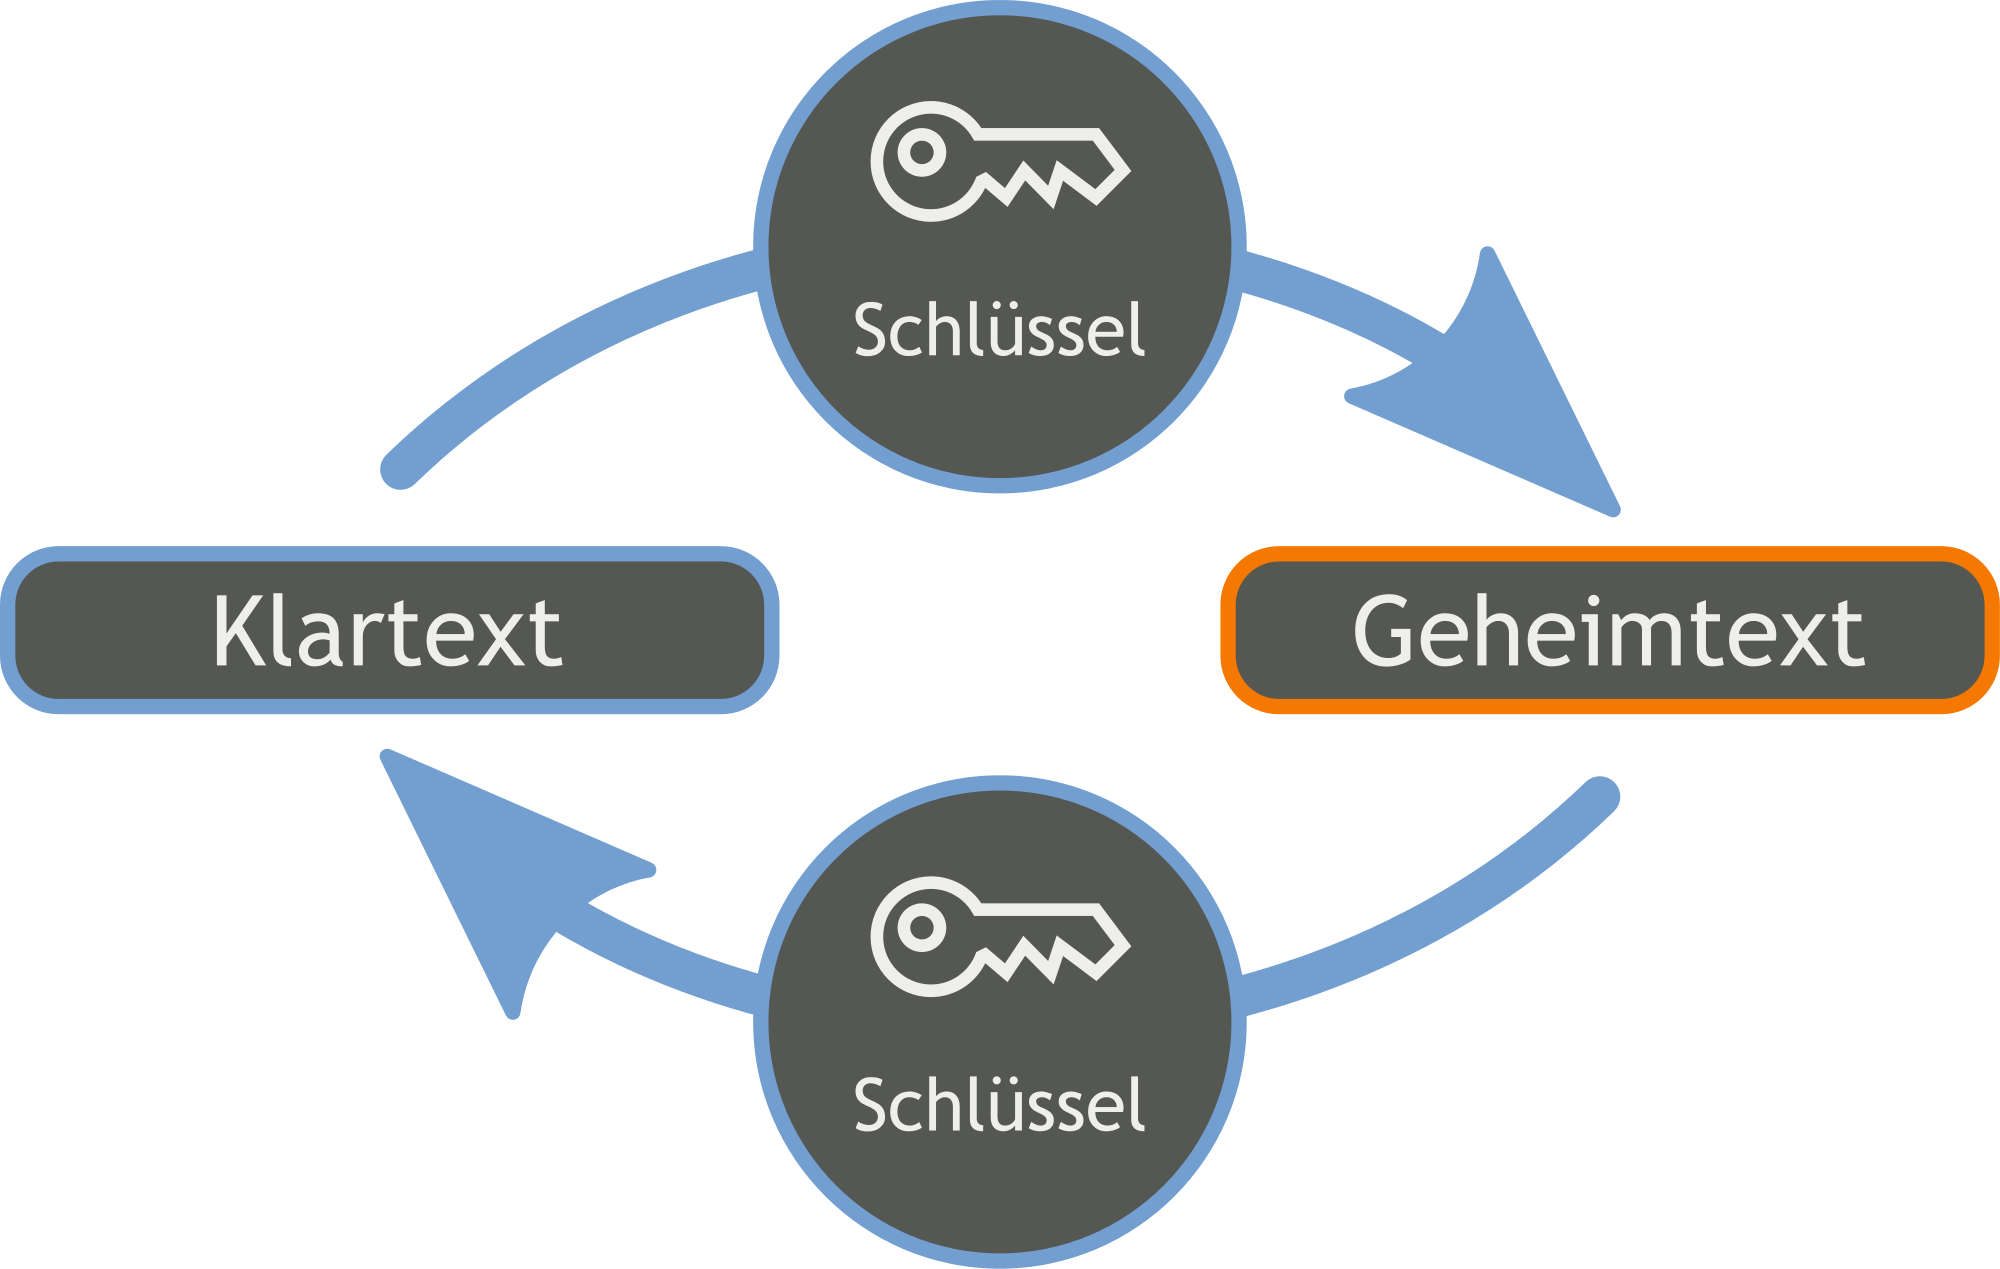
\includegraphics[scale=0.7,natwidth=629,natheight=225]{symm_shema.png} %ref link wikipedia
\end{center}
Abb. 1: Prinzip symmetrischer Verschlüsselung

% Daniel
\subsection{Stromchiffren}
Stromchiffren verarbeiten immer jedes Bit einer Nachricht einzeln, also ein Bit rein ein Bit raus. Dabei kommt es zu dem Problem, dass der Empfänger nicht weiß, an welcher Stelle der Sender im Strom gerade ist und falls mal ein Teil der Nachricht bei der Übertragung verloren gehen sollte, vergrößert es das Problem nur noch.

\subsection{Blockchiffren}
Blockchiffren verarbeiten immer eine bestimmte Menge an Bits einer Nachricht in einem ganzen Block. Das Problem dabei ist, dass manchmal ein Block zu klein ist und somit die Verschlüsselung überhaupt nicht stattfinden kann. Die größe der Blöcke hängt vom Schlüssel ab. So wird zum Beispiel bei AES128 mit 128-Bit Schlüsseln gearbeitet und somit in 128-Bit Blöcken verschlüsselt.

\subsection{Sicherheit}\label{symm:secu}
Die Sicherheit von symmetrischen Verfahren hängt stark vom Schlüssel ab. Ein zu kurzer Schlüssel zum Beispiel könnte schnell, durch ausprobieren, errechnet werden und somit wäre die Kommunikation nicht mehr sicher. Deshalb ist ein langer Schlüssel\footnote{Heutzutage 1024 Bit.} wichtig, allerdings bringt auch ein langer Schlüssel nichts, wenn er eines Tages an die Öffentlichkeit geraten sollte. Denn dann könnte jeder, der die entsprechenden Geheimdaten gesammelt hat, den Schlüssel nutzen, um diese zu entschlüsseln. Es ist also sehr wichtig, dass der Schlüssel geheim bleibt. Deshalb ist die Schlüsselverteilung (\cite{schlusselverteilung}) auch ein wichtiger Punkt, wenn man über Sicherheit von symmetrischen Verfahren redet. Die Schlüsselverteilung findet heutzutage häufig über asymmetrische Verfahren statt oder durch direkten Kontakt der Kommunikationspartner.

\newpage
\section{Asymmetrische Verschlüsselung}\label{asymm}
Asymmetrische Verschlüsselung ist im Vergleich zu symmetrischer Verschlüsselung noch recht jung. Im Jahr 1975 veröffentlichten Martin Hellman und Whitfield Diffie ihr Diffie-Hellman-Schlüsselaustausch-Protokoll und damit die ersten Ideen zur asymmetrischen Verschlüsselung. Das erste wirkliche asymmetrische Verschlüsselungsverfahren wurde allerdings erst 1977 von R. L. Rivest, A. Shamir und L. M. Adleman erfunden. Es erhielt den Namen RSA und ist bis heute immer noch eins der bekanntesten und am häufigsten genutzten Verfahren. Andere bekannte Verfahren sind McEliece(1978), Rabin(1979), Chor-Rivest(1984) und Elgamal(1985). (vgl. \cite{asymm_gesch} Geschichte)
\subsection{Prinzip asymmetrischer Verschlüsselung}\label{asymm:prinzip}
Asymmetrische Verschlüsselung ist das Gegenstück zu symmetrischer Verschlüsselung, denn hier gibt es nicht nur einen Schlüssel, der für Ver- und Entschlüsselung gebraucht wird, sondern jede Partei einer Kommunikation besitzt einen unterschiedlichen öffentlichen Schlüssel, welcher für jeden zugänglich ist, und einen privaten Schlüssel, welcher nur der jeweiligen Partei bekannt ist. Wenn jetzt zum Beispiel Partei A einer zweiten Partei B eine Nachricht schicken will, fragt Partei A bei Partei B nach ihrem öffentlichen Schlüssel. Die Übertragung dieses Schlüssels muss nicht sicher sein. Nach dem sie diesen erhalten hat, verschlüsselt Partei A ihre Nachricht mit diesem öffentlichen Schlüssel über einen Verschlüsselungsalgrorithmus und erhält einen Geheimtext, den sie selber nicht mehr entschlüsseln kann. Dieser Geheimtext wird dann zu Partei B geschickt und diese kann dann mit Hilfe ihres privaten Schlüssels und dem passenden Entschlüsselungsalgorithmus den Geheimtext entschlüsseln. Die Ver- und Entschlüsselungsalgorithmen, welche Partei A und B benutzen, benutzen eine Einwegfunktion mit Falltür (Definition in Kapitel \ref{oneway_trapdoor}), welche als Falltürinformation den jeweiligen privaten Schlüssel benutzt. (\cite{delfs_knebl} S.23 - 24) \newline Folgende Grafik verdeutlicht dieses Schema:
\begin{center}
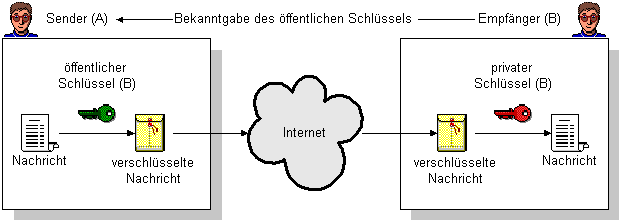
\includegraphics[scale=0.7,natwidth=622,natheight=222]{asymm_shema.png} %ref link wikipedia
\end{center}
Abb. 2: Prinzip asymmetrischer Verschlüsselung
\subsection{Digitale Signaturen}\label{asymm:sign}
Signaturen werden mit Hilfe der Einwegfunktion $f(x)$, welche die Ver- /Entschlüsselungsalgorithmen benutzen, erstellt. Die Einwegfunktion muss allerdings eine zusätzliche Eigenschaft haben, sie muss bijektiv sein. Das heißt, dass es für jeden $x$ Wert, nur genau einen $y$ Wert gibt und für jeden $y$ Wert genau einen $x$ Wert.
Wenn jetzt Partei A eine Nachricht $n$ an Partei B schicken will, kehrt Partei A die Funktion $f(x)$ mit ihrem privaten Schlüssel um und signiert dann mit $f^{-1}(x)$ die Nachricht $n$ und erhält die Signatur $s = f^{-1}(n)$. Diese wird dann an Partei B geschickt und die kann dann mit $f(s) = n$ und dem öffentlichem Schlüssel von Partei A, die erhaltene Nachricht verifizieren. Partei B weiß nun, dass Partei A die Nachricht geschickt haben muss, da nur sie $f^{-1}(x)$ berechnen konnte. (\cite{delfs_knebl} S.24 - 25)
\subsection{Sicherheit} % Daniel
Asymmetrische Verschlüsselungsverfahren haben das Problem der Schlüsselverteilung nicht, weshalb sie gegenüber symmetrischen Verfahren in dem Punkt sicherer sind. Des Weiteren gibt es bis jetzt keine effizienten Algorithmen, um die beschriebenen Einwegfunktionen umzukehren ohne die entsprechenden Geheiminformationen zu kennen. Die einzige Möglichkeit dafür ist ausprobieren und das dauert zu lange ($2^{n}$ Möglichkeiten), wenn der Schlüssel lang genug ist. Durch Signaturen gewinnen asymmetrische Verfahren auch noch an Sicherheit. (siehe Kapitel \ref{crypt:goals} und \ref{asymm:sign})



\section{Merkle-Hellman-Kryptosystem}\label{mhk}
Das asymmetrische Merkle-Hellman-Kryptosystem wurde 1978 von Ralph Merkle und Martin Hellman erfunden und ist eins der ersten asymmetrischen Kryptosysteme. Es verwendet anders als andere Verfahren (z.B.: RSA) keine digitalen Signaturen. Das Verfahren basiert auf dem Rucksackproblem, welches in Kapitel \ref{rucksack} erläutert wird.

%vergleiche bio merkle & hellman
\subsection{Über die Erfinder}
Ralph Merkle wurde 1952 in Carlifornien geboren. Er schloss 1974 sein Informatikstudium in UC Berkley ab. Im Jahr 1974 stellte er seinen Professoren seine Entdeckung zum kryptographischen Schlüsselaustausch, heute bekannt als Merkle's Puzzles, vor. Allerdings hatten sie kein weiteres Interesse an seiner Idee. Doch als er auf Whitfield Diffie und Matrin Hellman traf, nahm er seine Idee wieder auf und zusammen entwickelten sie das Merkle-Hellman-Kryptosystem. Heutzutage ist Merkle in der Nanotechnologie-branche tätig. (vgl. \cite{ralph_bio})  \newline Martin Hellman wurde 1945 in New York geboren. Er schloss sein Studium in Elektrotechnik 1969 an der Standford University ab. Im Jahre 1976 publizierte er zusammen mit Whitfield Diffie einen Artikel über den Diffie-Hellman Schlüsselaustausch und erste Ideen zur asymmetrischen Verschlüsselung. Heutzutage ist Hellman Professor in Standford im Fach Elektrotechnik. (vgl. \cite{martin_bio})

\subsection{Das Rucksackproblem}\label{rucksack}
Da das Merkle-Hellman-Kryptosystem auf dem Rucksackproblem basiert wird es in diesem Unterkapitel erläutert. \newline Das Rucksackproblem ist leicht mit einem Beispiel zu erklären: Stellen sie sich vor man hat einen Rucksack, der nur mit einer bestimmten Menge an Gewicht voll gepackt werden kann. Des Weiteren liegen neben dem Rucksack ein paar Gewichte, welche nicht gleich schwer sind und jeweils einen bestimmten Wert haben. Welche Gewichte kommen in den Rucksack, so dass die Gewichtsgrenze nicht überschritten wird und der maximale Wert (Die Summe aller Werte, der Gewichte im Rucksack) erzielt wird? \newline
Hier ein Beispiel:
\begin{center}
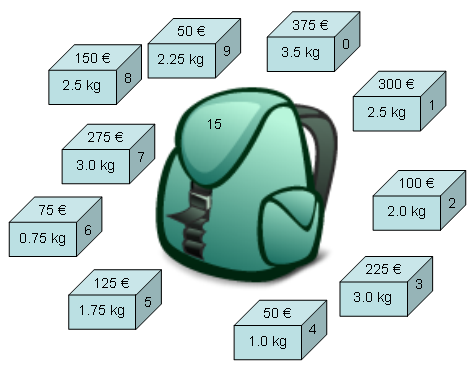
\includegraphics[scale=0.1,natwidth=2000,natheight=1733]{rucksackproblem.png} %ref link wikipedia
\end{center}
Abb. 3: Rucksackproblem Beispiel
Der abgebildete Rucksack kann maximal 15 kg tragen. Um ihn herum liegen 5 Gewichte mit den jeweiligen Werten in Dollar, aber welche werden eingepackt? Um dies herauszufinden werden alle Möglichkeiten, inklusive keine und alle Gewichte im Rucksack, durchprobiert. Dann wird geschaut, welche Möglichkeiten unter der Gewichtsgrenze liegen und den größten Wert erzielen. Für $n$ Gewichte gibt es $2^{n}$ verschiedene Möglichkeiten. Für das Beispiel gibt es also $2^{5} = 32$ Möglichkeiten. Das sind noch nicht viele und lässt sich deshalb schnell berechnen. Hat man jetzt allerdings weitaus mehr Gewichte, lässt sich das Problem nicht mehr effizient lösen. Es gibt eine Ausnahme, welche für das Merkle-Hellman-Kryptosystem sehr wichtig ist, diese wird in den nächsten Unterkapiteln erklärt. (\cite{knapsack})

%algorithmus
\subsection{Verfahren}
Die folgenden Unterkapitel erklären die Schlüsselerzeugung, die Verschlüsselung und Entschlüsselung des Merkle-Hellman-Kryptosystems. (\cite{merklehellman_neer})
\subsubsection{Schlüsselerzeugung}
Bei der Schlüsselerzeugung wird zuerst der private Schlüssel generiert und dieser muss ein stark wachsender Vektor sein. Das spielt bei der Entschlüsselung eine entscheidene Rolle. Außerdem muss er eine Länge von acht Elementen haben, da ein Buchstabe im Binärcode acht Bits hat. Ein solcher privater Schlüssel $S_p$ könnte folgendermaßen aussehen:
\begin{center}
$S_p=\{44,45,90,180,360,720,1440,2880\}$
\end{center}
Nachdem der private Schlüssel generiert wurde, wird der öffentliche Schlüssel erstellt. Dazu benötigt man zwei weitere Zahlen $m,n$, mit $m,n \in \mathbb{Z}$. $m$ wird so gewählt, dass sie größer ist als die Summe aller Elemente des privaten Schlüssels. Im Fall von $S_p$, mit $k$ als die Anzahl aller Elemente:
\begin{equation*}
m > \sum_{i=0}^{k-1} S_p[i]
\end{equation*}
n wird zufällig gewählt, allerdings so, dass der $ggT(m, n) = 1$ ist.
Für unser Beispiel wählen wir $m = 16511$ und $n = 11111$. Um jetzt den öffentlichen Schlüssel $S_{"o}$ zu erstellen, rechnet man für jedes Element $i$:
\begin{equation*}
S_{"o}[i]=(S_p[i] \times n)\; mod \; m
\end{equation*}
Für unseres Beispiel ergibt sich dann der öffentliche Schlüssel:
\begin{center}
$S_{"o}=\{10065,4665,9330,2149,4298,8596,681,1362\}$
\end{center}

\subsubsection{Verschlüsselung}
Bei der Verschlüsselung wird der Klartext $T_k$ erst in Binärcode umgewandelt. Für das Beispiel wählen wir ''Hallo'' als Klartext.
\begin{center}
%$T_k = \{\{0,1,0,0,1,0,0,0\},\{0,1,1,0,0,0,0,1\},\{0,1,1,0,1,1,0,0\},\{0,1,1,0,1,1,0,0\},\{0,1,1,0,1,1,1,1\}\}$
$T_k = \{01101000, 01100001, 01101100, 01101100, 01101111\}$
\end{center}
Nun wird jedes Bit von jedem Element von $T_k$ mit jedem Element von $S_{"o}$ multipliziert und diese jeweils immer acht Produkte werden addiert, so erhält man die einzelnen ''Geheimbuchstaben'', welche zusammen den Geheimtext $T_g$ ergeben.
Für unser Beispiel:
\begin{center}
$T_g=\{18293,15357,26889,26889,28932\}$
\end{center}
\subsubsection{Entschlüsselung}
Zum Entschlüsseln benötigt man $S_p,n,m$ und das modulare Inverse $m^{-1}$ von $m$ und $n$, welches mit dem erweiterten euklidischen Algorithmus (siehe Kapitel \ref{exteuk}) berechnet wird.
Für unser Beispiel gilt $m^{-1} = 584$.
Nun wird, um den Klartext zu erhalten, zuerst jedes Element $i$ von $T_g$ mit $m^{-1}$ multipliziert und mit Rest durch m dividiert.
\begin{equation*}
T_g[i] = (T_g[i] \times m^{-1})\; mod \; m
\end{equation*}
Für das Beispiel ergibt sich die transformierte Version von $T_g$:
\begin{center}
$T_g=\{495,3015,1215,1215,5535\}$
\end{center}
Danach kommt der Teil in dem die erwähnte Ausnahme des Rucksackproblems wichtig wird.
Analog stehen hier die Elemente des privaten Schlüssel $S_p$ für die Gewichte, welche alle 1 kg wiegen und den Wert $S_p[i]$ haben. Die Gewichtsgrenze des Rucksacks liegt bei 8 kg, also würden theoretisch alle Gewichte hinein passen, allerdings wird hier nicht probiert den maximalen Wert zu erreichen, sondern es wird probiert die Werte in $T_g$ zu erreichen und deshalb ist es wichtig, dass der private Schlüssel ein stark wachsender Vektor ist, denn nur dann ist das Rucksackproblem schnell zu lösen. Man erhält als Lösung den Klartext in Binärcodes, in denen eine 1 für ein zutreffendes Element im Schlüssel zur Lösung steht und eine 0 für ein nicht zutreffendes Element. \newline Hier das ganze für den ersten Buchstaben am Beispiel:

Für $T_g[0]$ soll eine Lösung aus den Werten von $S_p$ gefunden werden, um den ersten Buchstaben in binär zu erhalten.

\begin{equation*}
T_g[0] = 495
\end{equation*}
Die Lösung lautet $01101000$, da:
\begin{equation*}
(0 \cdot 44) + (1 \cdot 45) + (1 \cdot 90) + (0 \cdot 180) + (1 \cdot 360)  + (0 \cdot 720 )+ (0 \cdot 1440 )+ (0 \cdot 2880) = 495
\end{equation*}
Dasselbe muss jetzt für jedes Element in $T_g$ getan werden und man erhält den Klartext:
\begin{equation*}
T_k = \{01101000, 01100001, 01101100, 01101100, 01101111\}
\end{equation*}

\subsection{Sicherheit}
Zur generellen Sicherheit des Verfahrens sollte man sagen, dass solange $m, n, m^{-1}, S_p$ nicht bekannt sind, es schwer sein sollte das System zu kompromittieren. Allerdings hat Adi Shamir, einer der Erfinder des RSA-Vefahrens, es 1982 trotzdem geschafft. Shamirs Methode, zum kompromittieren des Verfahrens ist sehr komplex und würde den Rahmen dieser Facharbeit definitiv sprengen. Des Weiteren beinhaltet das Merkle-Hellman-Kryptosystem keine Methoden zum Signieren, was mit Hinblick auf die Sicherheit ein großes Problem ist, denn dadurch sind zwei Ziele der Verschlüsselung (Authentizität und Nichtabstreitbarkeit) nicht erreicht. %merkle-hellman-knapsack-based-public-key-method.pdf

\newpage
\section{Fazit}
Die Ziele dieser Arbeit sind, den Lesern ein grundsätzliches Verständnis über Verschlüsselung zu vermitteln und im Besonderen asymmetrische Verschlüsselungsverfahren am Beispiel des Merkle-Hellman-Kryptosystem zu verstehen und
auch wenn das Merkle-Hellman-Kryptosystem nicht sicher ist, ist es dennoch sehr interessant, da es eins der ersten asymmetrischen Verfahren ist und das Rucksackproblem auch in anderen Verfahren zum Einsatz kommt, weil es an sich gut für die Kryptographie geeignet ist. Die mir bis jetzt bekannten Leser der Arbeit haben mir mitgeteilt, dass sie nun das grundsätzliche Verständnis erlangt haben.

Was mich angeht, hat mich die Bearbeitung dieses Themas weiter gebracht, da ich viel über das ganze Thema recherchieren musste und somit viel gelernt habe. Außerdem hat es mich in meinen Plänen ein Studium, in die mathematische Richtung zu wählen nur noch bestärkt.
\newpage

\begin{flushleft}
\bibliography{facharbeit}
\end{flushleft}
\large
\textbf{Abbildungsverzeichnis} \newline
\normalsize
\begin{flushleft}
Abb. 1: \url{http://ddi.cs.uni-potsdam.de/Lehre/e-commerce/elBez2-5/des.gif} (8.3.2015) \newline
Abb. 2: \url{http://ddi.cs.uni-potsdam.de/Lehre/e-commerce/elBez2-5/rsa1.gif} (8.3.2015) \newline
Abb. 3: \url{http://upload.wikimedia.org/wikipedia/commons/thumb/f/fd/Knapsack.svg/2000px-Knapsack.svg.png} (8.3.2015)
\end{flushleft}
\newpage
\section{Erklärung}
Hiermit erkläre ich, dass ich die vorliegende Arbeit selbstständig und ohne fremde Hilfe verfasst und keine als die im Literaturverzeichnis angegebenen Hilfsmittel verwendet habe. \newline
Insbesondere versichere ich, dass ich alle wörtlichen und sinngemäßen Übernahmen aus anderen Werken als solche kenntlich gemacht habe. \newline

\begin{tabular}{lp{2em}l}
 \hspace{5cm}   && \hspace{4cm} \\\cline{1-1}\cline{3-3}
 Ort, Datum     && Unterschrift
\end{tabular}
\end{document}

